% The first argument is the \documentclass, which tells latex which template
% we're using to build this document. It's usually safe to just use "article".
\documentclass{article}

% include some packages...
\usepackage{fullpage} % change settings for a smaller margin
\usepackage{graphicx} % gives access to the \includegraphics commands
\usepackage{amsfonts}
\usepackage{float}
\usepackage{enumitem}
\usepackage{caption}
\usepackage[export]{adjustbox}
\usepackage{bookmark}
\graphicspath{{./images/}}

% tell Latex to use no paragraph indentation, but leave some space between
% paragraphs
\setlength{\parindent}{0in}
\setlength{\parskip}{0.1in}

\newcommand{\tib}[1]{\textit{\textbf{#1}}}
\newcommand{\code}[1]{\texttt{#1}}

% these commands merely set the values for the title/date/author; they don't put
% them in the document... see \maketitle below
\title{CS Department Automated Information Timeline \\ Assignment 9.1: Component Diagram}
\date{\today}
\author{Matthew Hays, Pawan Bhandari, Sarah Faron, Tim Klimpel \\ The Incredibles}

% all document content goes between \begin{document} and \end{document}
\begin{document}

% this command actually creates the title/date/author in the document
\maketitle
\newpage
\tableofcontents
\listoffigures
\newpage
\section{Introduction}
\subsection{Purpose}
The purpose of this assignment is to collaborate as a team and create a component diagram of the CS Department Automated Information Timeline project. Team members worked together and created the component diagrams which is presented in Section 2 of this document.

\section{Component Diagram}

\begin{figure}[H]
    \centering
    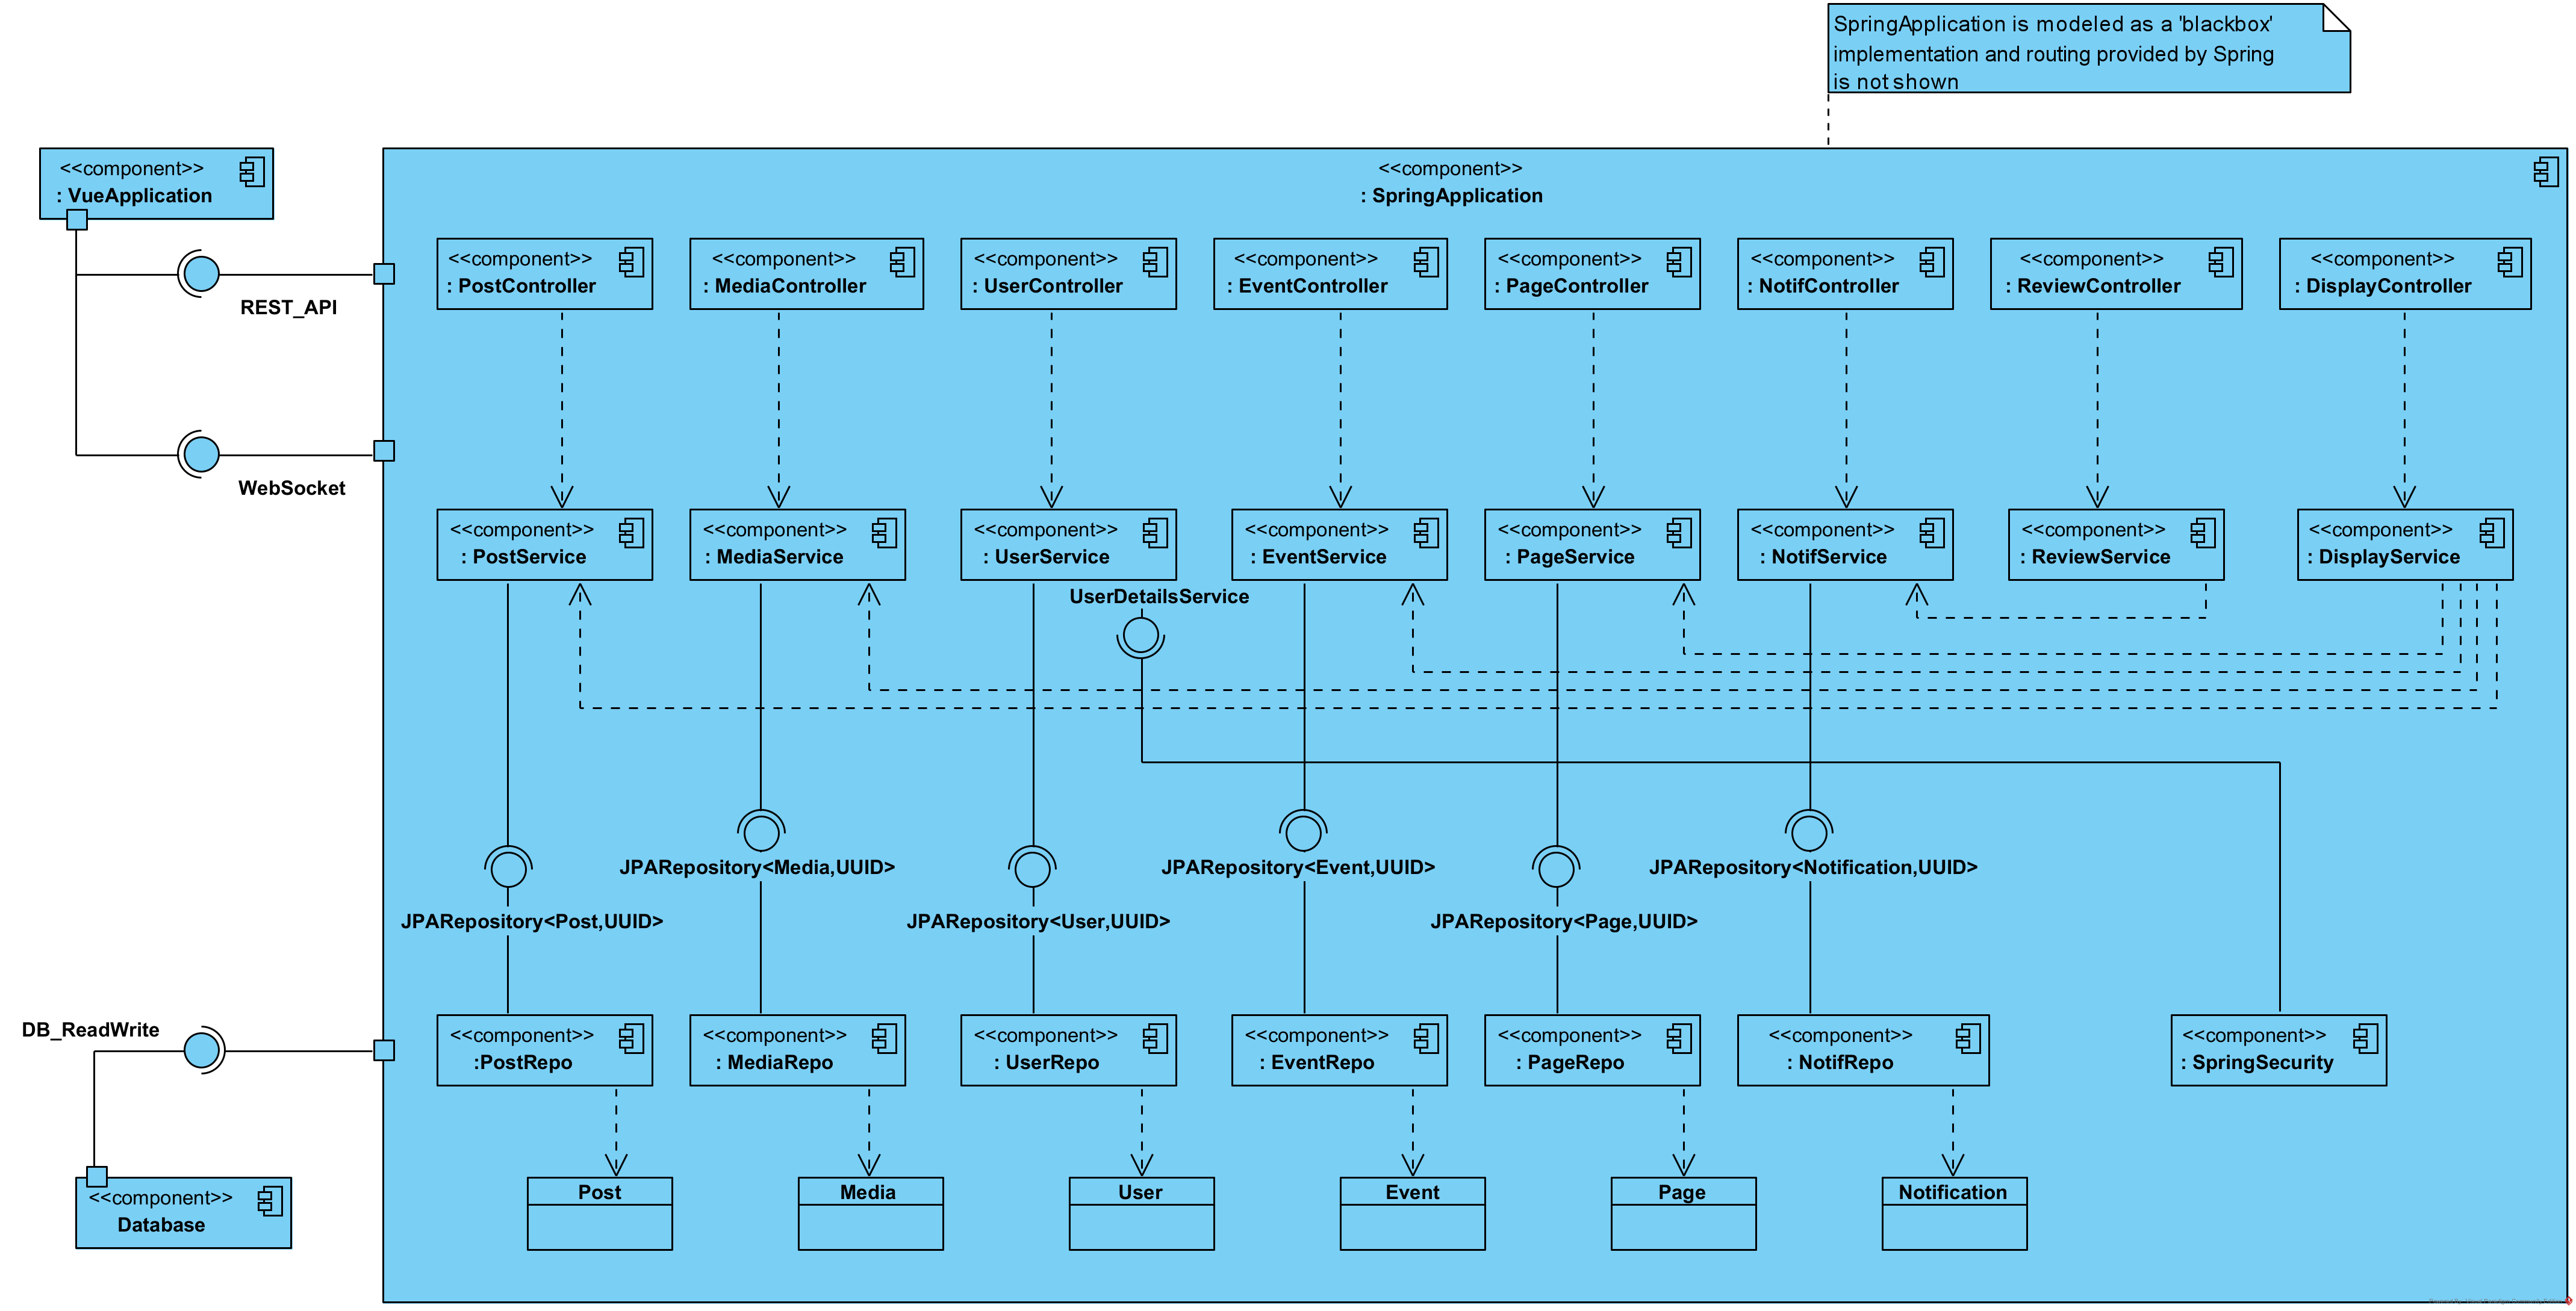
\includegraphics[width=1.05\textwidth]{images/Component_Diagram.png}
    \centering
    \caption{Component Diagram}
\end{figure}

\end{document}